\documentclass[12pt,letterpaper]{article}
\usepackage{fullpage}
\usepackage[top=2cm, bottom=4.5cm, left=2.5cm, right=2.5cm]{geometry}
\usepackage{amsmath,amsthm,amsfonts,amssymb,amscd}
\usepackage{lastpage}
\usepackage{enumerate}
\usepackage{fancyhdr}
\usepackage{mathrsfs}
\usepackage{xcolor}
\usepackage{graphicx}
\usepackage{listings}
\usepackage{hyperref}
\usepackage{tikz}
\usepackage{xfrac}
\usepackage{nicefrac}
\usepackage{xcolor}

\usetikzlibrary{shapes.geometric,fit}
\usetikzlibrary{patterns}

\hypersetup{
    colorlinks=true,
    linkcolor=blue,
    linkbordercolor={0 0 1}
}

\setlength{\parindent}{0.0in}
\setlength{\parskip}{0.05in}

\newcommand\course{ECON 3211}
\newcommand\hwnumber{8}
\newcommand\NetIDa{dc3451}
\newcommand\NetIDb{David Chen}

\theoremstyle{definition}
\newtheorem*{statement}{Statement}
\newtheorem*{claim}{Claim}
\newtheorem*{theorem}{Theorem}

\newcommand{\contra}{\Rightarrow\!\Leftarrow}
\newcommand{\Lag}{\mathcal{L}}

\pagestyle{fancyplain}
\headheight 35pt
\lhead{\NetIDa}
\lhead{\NetIDa\\\NetIDb}
\chead{\textbf{\Large Problem Set \hwnumber}}
\rhead{\course \\ \today}
\lfoot{}
\cfoot{}
\rfoot{\small\thepage}
\headsep 1.5em

\begin{document}

\section*{Problem 1}

\subsection*{a)}

Country 1:

\begin{align*}
  Q_D &= 20 - P \\
  \epsilon_D &= \frac{dQ}{dP} \cdot \frac{P}{Q} \\
      &= -1(\frac{P}{20 - P}) \\
  10 &= P^*(1 - \frac{20 - P^*}{P^*}) \\
      &= P^* - 20 + P^* \\
      &= 2P^* - 20 \\
  P^* &= 15 \\
\end{align*}


Country 2:

\begin{align*}
  Q_D &= (\frac{A}{P})^2 \\
  \epsilon_D &= (-\frac{2A^2}{P^3})(\frac{P^3}{A^2}) \\
      &= -2 \\
  10 &= P^*(1 - \frac{1}{2}) \\
  P^* &= 20 \\
\end{align*}

Country 3:

\begin{align*}
  Q_D &= (\frac{A}{P})^3 \\
  \epsilon_D &= (-\frac{3A^3}{P^4})(\frac{P^4}{A^3}) \\
      &= -3 \\
  10 &= P^*(1 - \frac{1}{3}) \\
  P^* &= 15 \\
\end{align*}
We can compute the new price that the firm has by taking $MR = 11$.

\subsection*{b)}

Country 1:

\begin{align*}
  Q_D &= 20 - P \\
  \epsilon_D &= \frac{dQ}{dP} \cdot \frac{P}{Q} \\
      &= -1(\frac{P}{20 - P}) \\
  11 &= P^*(1 - \frac{20 - P^*}{P^*}) \\
      &= P^* - 20 + P^* \\
      &= 2P^* - 20 \\
  P^* &= 15.5 \\
\end{align*}

The new price is increased by $\frac{1}{2}$ of the tax, so the incidence is
$50-50$ on the consumers and the firm.

Country 2:

\begin{align*}
  Q_D &= (\frac{A}{P})^2 \\
  \epsilon_D &= (-\frac{2A^2}{P^3})(\frac{P^3}{A^2}) \\
      &= -2 \\
  11 &= P^*(1 - \frac{1}{2}) \\
  P^* &= 22 \\
\end{align*}

The new price is increased by twice the tax, so the incidence is $200\%$ on
consumers.

Country 3:

\begin{align*}
  Q_D &= (\frac{A}{P})^3 \\
  \epsilon_D &= (-\frac{3A^3}{P^4})(\frac{P^4}{A^3}) \\
      &= -3 \\
  11 &= P^*(1 - \frac{1}{3}) \\
  P^* &= 16.5 \\
\end{align*}

The new price is increased by 1.5 times the tax, so the incidence is $150\%$ on
consumers.

\section*{Problem 2}

\subsection*{a), b)}

\begin{center}
  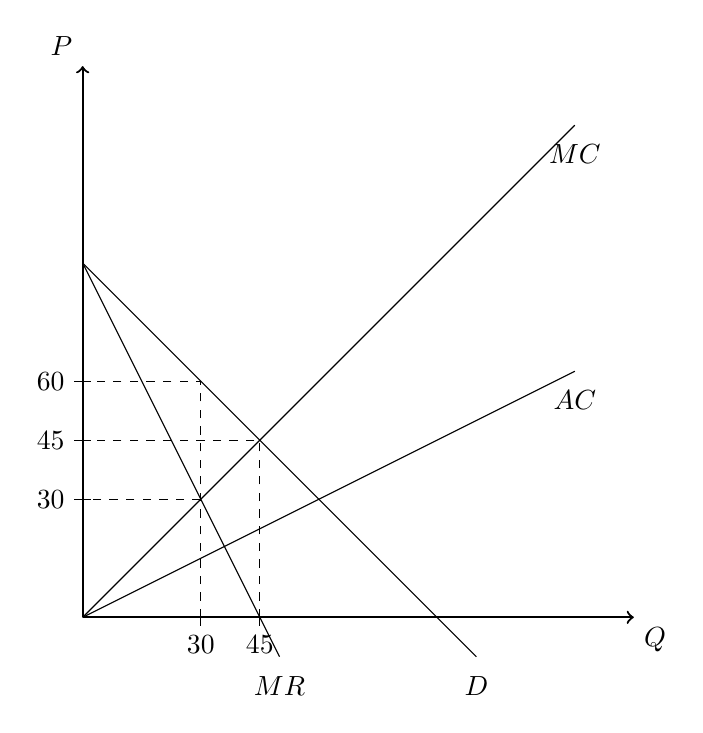
\begin{tikzpicture}[
    dot/.style={shape=circle, inner sep=2pt, draw, node contents=},
    circ/.style={shape=circle, inner sep=2pt, draw, fill}]
    \draw[thick,->] (0,0) -- (7,0) node[anchor=north west] {$Q$};
    \draw[thick,->] (0,0) -- (0,7) node[anchor=south east] {$P$};

    \draw (3pt,3cm) -- (-3pt,3cm) node[anchor=east] {$60$}; 
    \draw (1.5cm,3pt) -- (1.5cm,-3pt) node[anchor=north] {$30$};
    \draw (3pt,2.25cm) -- (-3pt,2.25cm) node[anchor=east] {$45$}; 
    \draw (3pt,1.5cm) -- (-3pt,1.5cm) node[anchor=east] {$30$}; 
    \draw (2.25cm,3pt) -- (2.25cm,-3pt) node[anchor=north] {$45$};
    % \draw (3pt,6.4cm) -- (-3pt,6.4cm) node[anchor=east] {$32$}; 
    % \draw (3pt,0.4cm) -- (-3pt,0.4cm) node[anchor=east] {$2$}; 
    % \draw (3pt,2cm) -- (-3pt,2cm) node[anchor=east] {$10$}; 
    % \draw (3pt,3.1cm) -- (-3pt,3.1cm) node[anchor=east] {$15.5$}; 
    \draw[domain=0:100,scale=0.05,smooth,variable=\x] plot ({\x},{90 - \x}) node[label=below:{$D$}]{};
    \draw[domain=0:50,scale=0.05,smooth,variable=\x] plot ({\x},{90 - 2*\x}) node[label=below:{$MR$}]{};
    \draw[domain=0:125,scale=0.05,smooth,variable=\x] plot ({\x},{0.5*\x}) node[label=below:{$AC$}]{};
    \draw[domain=0:125,scale=0.05,smooth,variable=\x] plot ({\x},{\x}) node[label=below:{$MC$}]{};
    % \draw[domain=25:125,scale=0.05,smooth,variable=\x] plot ({\x},{\x-25}) node[label=below:{$MC$}]{};
    \draw[dashed] (1.5, 0) -- (1.5, 3) -- (0, 3);
    \draw[dashed] (1.5, 1.5) -- (0, 1.5);
    \draw[dashed] (2.25, 0) -- (2.25, 2.25) -- (0, 2.25);
  \end{tikzpicture}
\end{center}

The socially optimal price is $45$, the socially optimal quantity is $45$. The
profit maximizing price is $60$, the profit maximizing quantity is $30$.

\subsection*{c)}

The imposition of a tax on profits does not actually change the equilibrium (the
profit maximizing price and quantity) as the firm considers it much like a lump
sum tax as it does not change $MC$ or $MR$. Then, it also does not reduce
deadweight loss.

\subsection*{d)}

Perfect price discrimination would allow the firm to capture all of consumer
surplus, meaning that they would produce at the socially optimal level in order
to maximize total surplus.

Thus, the price charged would be $45$, selling also $45$, for a profit of
$\frac{1}{2}(90)(45) = 2025$ ($1012.5$ if taxed at 50\%). The deadweight loss
would be 0.

\subsection*{e)}

To minimize deadweight loss, the government ought to use a subsidy;
specifically, a per-unit subsidy should increase production and lower prices,
bringing equilibrium closer to socially optimal levels.

\begin{center}
  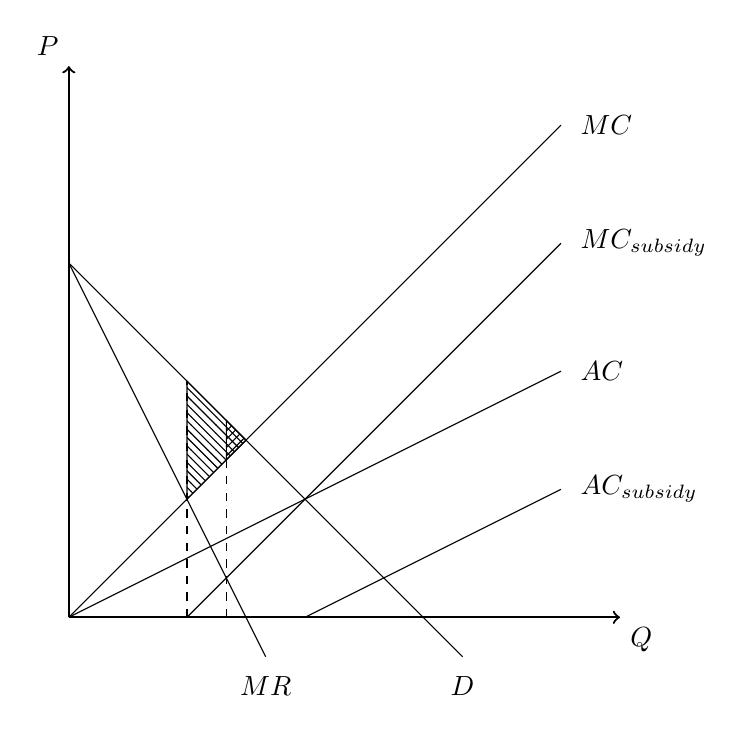
\begin{tikzpicture}[
    dot/.style={shape=circle, inner sep=2pt, draw, node contents=},
    circ/.style={shape=circle, inner sep=2pt, draw, fill}]
    \draw[thick,->] (0,0) -- (7,0) node[anchor=north west] {$Q$};
    \draw[thick,->] (0,0) -- (0,7) node[anchor=south east] {$P$};

    % \draw (3pt,3cm) -- (-3pt,3cm) node[anchor=east] {$60$}; 
    % \draw (1.5cm,3pt) -- (1.5cm,-3pt) node[anchor=north] {$30$};
    % \draw (3pt,2.25cm) -- (-3pt,2.25cm) node[anchor=east] {$45$}; 
    % \draw (3pt,1.5cm) -- (-3pt,1.5cm) node[anchor=east] {$30$}; 
    % \draw (2.25cm,3pt) -- (2.25cm,-3pt) node[anchor=north] {$45$};
    \draw[domain=0:100,scale=0.05,smooth,variable=\x] plot ({\x},{90 - \x}) node[label=below:{$D$}]{};
    \draw[domain=0:50,scale=0.05,smooth,variable=\x] plot ({\x},{90 - 2*\x}) node[label=below:{$MR$}]{};
    \draw[domain=0:125,scale=0.05,smooth,variable=\x] plot ({\x},{0.5*\x}) node[label=right:{$AC$}]{};
    \draw[domain=60:125,scale=0.05,smooth,variable=\x] plot ({\x},{0.5*\x - 30}) node[label=right:{$AC_{subsidy}$}]{};
    \draw[domain=0:125,scale=0.05,smooth,variable=\x] plot ({\x},{\x}) node[label=right:{$MC$}]{};
    \draw[domain=30:125,scale=0.05,smooth,variable=\x] plot ({\x},{\x-30}) node[label=right:{$MC_{subsidy}$}]{};
    \draw[pattern=north west lines] (1.5,1.5) -- (1.5,3) -- (2.25, 2.25) -- cycle;
    \draw[pattern=north east lines] (2,2) -- (2,2.5) -- (2.25, 2.25) -- cycle;
    \draw[dashed] (1.5, 0) -- (1.5, 3);
    \draw[dashed] (2, 0) -- (2, 2.5);
    % \draw[dashed] (1.5, 1.5) -- (0, 1.5);
    % \draw[dashed] (2.25, 0) -- (2.25, 2.25) -- (0, 2.25);
  \end{tikzpicture}
\end{center}

The area in northwest lines is old deadweight loss; the area in northeast lines
new deadweight loss after a subsidy of 30.

\section*{Problem 3}

\subsection*{a)}

The profit maximizing price is equal to $MC$, so $p = 1$. The maximizing fee is
equal to consumer surplus, so $F = \frac{1}{2}(4)(4) = 8$. They ought to charge
$F$ slightly less than this, so about $7.99$.

\subsection*{b)}

\begin{center}
  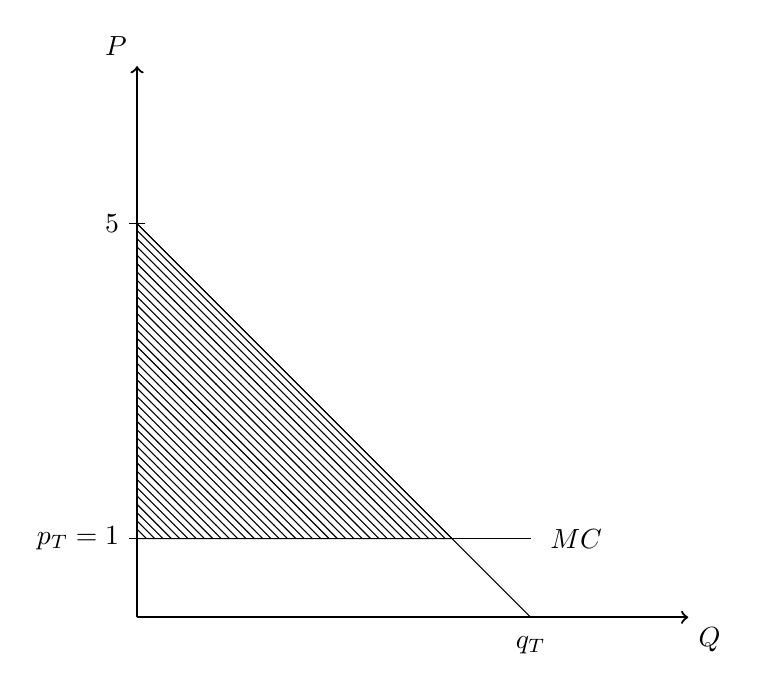
\begin{tikzpicture}[
    dot/.style={shape=circle, inner sep=2pt, draw, node contents=},
    circ/.style={shape=circle, inner sep=2pt, draw, fill}]
    \draw[thick,->] (0,0) -- (7,0) node[anchor=north west] {$Q$};
    \draw[thick,->] (0,0) -- (0,7) node[anchor=south east] {$P$};

    % \draw (3pt,3cm) -- (-3pt,3cm) node[anchor=east] {$60$}; 
    % \draw (1.5cm,3pt) -- (1.5cm,-3pt) node[anchor=north] {$30$};
    % \draw (3pt,2.25cm) -- (-3pt,2.25cm) node[anchor=east] {$45$}; 
    \draw (3pt,1cm) -- (-3pt,1cm) node[anchor=east] {$p_T = 1$}; 
    \draw (3pt,5cm) -- (-3pt,5cm) node[anchor=east] {$5$}; 
    % \draw (2.25cm,3pt) -- (2.25cm,-3pt) node[anchor=north] {$45$};
    \draw[domain=0:5,scale=1,smooth,variable=\x] plot ({\x},{5 - \x}) node[label=below:{$q_T$}]{};
    \draw[domain=0:5,scale=1,smooth,variable=\x] plot ({\x},{1}) node[label=right:{$MC$}]{};
    \draw[pattern=north west lines] plot (0,1) -- (4,1) -- (0,5) -- cycle;
    % \draw[dashed] (1.5, 1.5) -- (0, 1.5);
    % \draw[dashed] (2.25, 0) -- (2.25, 2.25) -- (0, 2.25);
  \end{tikzpicture}
\end{center}

The fee $F$ is equal to the shaded area.

\subsection*{c)}

Similar to above, profit maximizing $p_S = 1$, $F_S = \frac{1}{2}(3)(3) = 4.5$, or
slightly less at $4.49$.

\subsection*{d)}

The total profit is $2\frac{1}{2}(4-p)^2 + (p-1)((4-p) + (5-p)) = (4-p^2) +
(p-1)(9-2p)$. The FOC simplifies to $2p = 3 \implies p = 1.5$, with a profit
maximizing fee of $\frac{1}{2}(4-1.5)^2 = 3.125$, with a total of $9 - 2(1.5) =
6$ rides.

The senior's consumer surplus is 0. The teen's consumer surplus is
$\frac{1}{2}(5-1.5)^2 - 3.125 = 3$.

The deadweight loss is increased as the socially optimal price and quantity
is $1$ and $7$; thus, we have that DWL = $\frac{1}{2}(1)(0.5) = 0.25$.

\subsection*{e)}

\section*{Problem 4}
\subsection*{a)}
\subsubsection*{a.1}

We want that $MR(q_L) = MR(q_O + q_L), MR(q_O) = MC(q_O + q_L)$. We have that
$P_L = 30 - q_L$, $MR_L = 30 -2 q_L = 10 = MC$, so $q_L = 10$. Similarly, $P_O =
60 - 5q_O, MR_O = 60 - 10q_O = 10 = MC,$ so $q_O = 5$.

\subsubsection*{a.2}

$P_L = 30 -10 = 20, P_O = 60 - 5(5) = 35$.

\subsection*{b)}
\subsubsection*{b.1}

Let $Q$ be total demand, $Q^O$ total occasional demand, and $Q_L$ the total
lovers demand. Then, $Q^O = 100q_O = 1200 - 20P_O, Q^L = 100q_L = 3000 -
100P_L$.

\[
  Q = \begin{cases}
    Q^O & 30 < P \leq 60 \\
    Q^O + Q^L & 0 \leq P \leq 30
  \end{cases} = \begin{cases}
    1200 - 20P & 30 < P \leq 60 \\
    4200 - 120P & 0 \leq P \leq 30
  \end{cases}
\]

\subsubsection*{b.2,b.3}

We need that $MR = MC$. Since
\[
  P = \begin{cases}
    60 - \frac{Q}{20} & 0 \leq Q \leq 600 \\
    35 - \frac{Q}{120} & Q \geq 600
  \end{cases}
\],

we have that
\[
  MR = \begin{cases}
    60 - \frac{Q}{10} & 0 \leq Q \leq 600 \\
    35 - \frac{Q}{60} & Q \geq 600
  \end{cases}
\]


We have two possibilities; if they only sell to occasional customers, then $60 -
\frac{1}{10}Q = 10 \implies Q = 500, P = 60 -\frac{500}{20} = 35$.  If the sell
to both, then $35 - \frac{1}{60}Q = 10 \implies Q = 1500, P = 35 -
\frac{1500}{120} = 22.5$.

Since $\pi_O = 35(500) - 500(10) - FC = 12500 - FC, \pi_B = 22.5(1500) -
1500(10) - FC = 18750 - FC$. Thus, they sell to both and $P^* = 22.50, Q^* = 1500$.


\subsubsection*{b.4}

In tne price monopoly, $P = 22.5, Q = 1500, \pi = 18750 - FC$. In market
segmentation, $P_O = 35, Q_O = 500, P_L = 20, Q_L = 1000, \pi_{seg} = (20)1000 +
35(500) - 10(1500) - FC = 22500 - FC$.

We can see that segmenting the market has the occasional customers facing a
higher price, so they lose, but the opera lovers gain because they face a lower
price. The monopolist also gains because they increase total profit.

\subsection*{c)}
\subsubsection*{c.1}

The profit maximizing behavior of the firm is that they will actively target the
high paying audience with tickets and the more frequent, poorer customers the
subscription.

The subscription will be a two-part tariff with constant marginal cost; as
before there will be 20 such members in the market, so $n = 20$. The amount
charged, then will be capturing the totality of surplus, which is computed to be
$20(10) + \frac{1}{2} 20(20) = 400$. Since they want have opera lovers be better
off than just buying nothing, they charge $S = 399$.

Then, as before, we have that the profit maximizing price in the infrequent
customer market is $P = 35$; further, this price means that opera lovers are
priced out, and therefore is the actual ticket price in the presence of the subscription.

\subsubsection*{c.2}

We see that since occasional customers only gain surplus by buying tickets and
opera lovers only gain surplus by buying the subscription, the occasional
customers buy tickets and the lovers buy subscriptions.

\section*{Problem 5}

\subsection*{a)}

\[
  \pi(Q_{US},Q_A) = p_{US}Q_{US} + p_AQ_A - 10(Q_{US} + Q_A) = p_{US}(60-p_{US})
  + p_A(60-2p_A) - 10(120 - p_{US} - 2p_A)
\]

In terms of quantity,

\[
  \pi(Q_{US},Q_A) = p_{US}Q_{US} + p_AQ_A - 10(Q_{US} + Q_A) = Q_{US}(60-Q_{US})
  + Q_A(30-\frac{1}{2}Q_A) - 10(Q_{US} + Q_A)
\]

\subsection*{b), c), d)}

Are b) and c) not the same problem?

\[
  \frac{\partial \pi}{\partial p_{US}} = 60 - 2p_{US} + 10 = 0 \implies p^*_{US} =
  35, Q^*_{US} = 25
\]

\[
  \frac{\partial \pi}{\partial p_A} = 60 - 4p_A + 20 = 0 \implies p^*_A = 20,
  Q^*_A = 20
\]

In terms of quantity,

\[
  \frac{\partial \pi}{\partial p_{US}} = 60 - 2Q_{US} - 10 = 0 \implies Q^*_{US} =
  25, p^*_{US} = 35
\]

\[
  \frac{\partial \pi}{\partial p_A} = 30 - Q_A - 10 = 0 \implies Q^*_A = 20,
  p^*_A = 20
\]

\subsection*{e)}
\begin{center}
  \begin{tikzpicture}[
    dot/.style={shape=circle, inner sep=2pt, draw, node contents=},
    circ/.style={shape=circle, inner sep=2pt, draw, fill}]
    \draw[thick,->] (0,0) -- (7,0) node[anchor=north west] {$Q_{US}$};
    \draw[thick,->] (0,0) -- (0,7) node[anchor=south east] {$p_{US}$};
    \draw (3pt,3.5cm) -- (-3pt,3.5cm) node[anchor=east] {$35$}; 
    \draw (3pt,1cm) -- (-3pt,1cm) node[anchor=east] {$10$}; 
    \draw (8cm+3pt,1cm) -- (8cm-3pt,1cm) node[anchor=east] {$10$}; 
    \draw (8cm+3pt,2cm) -- (8cm-3pt,2cm) node[anchor=east] {$20$}; 
    \draw (2.5cm,3pt) -- (2.5cm,-3pt) node[anchor=north] {$25$};
    \draw (10cm,3pt) -- (10cm,-3pt) node[anchor=north] {$20$};
    \draw[domain=0:65,scale=0.1,smooth,variable=\x] plot ({\x},{60 - \x}) node[label=below:{$D_{US}$}]{};
    \draw[domain=0:35,scale=0.1,smooth,variable=\x] plot ({\x},{60 - 2*\x}) node[label=below:{$MR_{US}$}]{};
    \draw[domain=0:55,scale=0.1,smooth,variable=\x] plot ({\x},{10}) node[label=right:{$MC$}]{};
    \draw[thick,->] (8,0) -- (15,0) node[anchor=north west] {$Q_A$};
    \draw[thick,->] (8,0) -- (8,7) node[anchor=south east] {$p_A$};
    \draw[domain=0:65,scale=0.1,smooth,variable=\x] plot ({\x + 80},{30 - \x / 2}) node[label=below:{$D_{A}$}]{};
    \draw[domain=0:35,scale=0.1,smooth,variable=\x] plot ({\x + 80},{30 - \x}) node[label=below:{$MR_{A}$}]{};
    \draw[domain=0:65,scale=0.1,smooth,variable=\x] plot ({\x + 80},{10}) node[label=right:{$MC$}]{};
    \draw[dashed] (2.5,0) -- (2.5,3.5) -- (0,3.5);
    \draw[dashed] (10,0) -- (10,2) -- (8,2);
  \end{tikzpicture}
\end{center}

The profit maximizing quantities and prices are marked with dashed lines.

\subsection*{f)}

If the WTO bans region codes, then the US will benefit and Aus will suffer, as
the company is incentivized to hold prices somewhere inbetween $p_{US}$ and $p_A$.

More specifically, we have that once solved, $Q_T = 120 - 3P \implies Q^* = 45,
P^* = 30$ if they sell to both, making $\pi = 900$ compared to $\pi = 625$ in
solely the American market. This then hurts the Australians and helps Americans.

\end{document}